\documentclass[openright,twoside,12pt]{book}
    \usepackage{upmhthesis}
    \usepackage{lipsum}
    % \usepackage[notref,notcite]{showkeys}
    % \usepackage{showframe}
    % \usepackage{draftwatermark}
    %     \SetWatermarkText{\textsc{Borrador}}
    %     \SetWatermarkScale{1}
    %     \SetWatermarkAngle{55}
    % ============================================================
    % THESIS INFORMATION
    % ============================================================
    \title{Diseño de interfaz cerebro-computadora aplicada al control inteligente del helicóptero \textit{Quanser}}
    \titleEN{Brain-computer interface design applied to the helicopter Quanser intelligent control}
    
    \subject{Diseño de un controlador para el modelo experimental de un helicóptero de 2GDL}
    
    \keywords{control, redes neuronales, quanser, wavelets, helicóptero}
    \keywordsEN{control, artificial neural networks, wavelets, quanser, multiresolution}

    \author{Ing. Oscar Federico García Castro}
    \authorEN{Eng. Oscar Federico García Castro}
    
    \faculty{Maestría en Ingeniería Aeroespacial}
    \facultyEN{Master in Aerospace Engineering}
    
    \university{Universidad Politécnica Metropolitana de Hidalgo}
    \universityEN{Hidalgo Metropolitan Polytechnic University}
    
    \degree{Maestro en Ingeniería Aeroespacial}
    \supervisor{M. en C. Marío Alejandro Vega Navarrete\\[3mm]
                Dr. Luis Enrique Ramos Velasco}
    \cityandyear{Tolcayuca, Hgo.\hfill Agosto, 2023}
    \date{agosto, 2023}
    \logouniversity{titlepage/UPMH Cut}
    \logoconacyt{titlepage/conacyt}
    \logofaculty{titlepage/mia}

    \makeatletter\hypersetup{
        pdftitle    = {\@title},
        pdfsubject  = {\@subject},
        pdfauthor   = {\@author},
        pdfkeywords = {\@keywords},
    }
    
    \newcommand{\Quanser}{\textit{Quanser}}
% ================================================================
% ================================================================
\begin{document}
% ================================================================
    \selectlanguage{spanish}
    \renewcommand\spanishtablename{Tabla}
    \renewcommand{\listtablename}{Lista de tablas}
    \renewcommand{\listfigurename}{Lista de figuras}
    \addtocontents{toc}{~\hfill\textbf{Página}\\[-0.5em]}
    
    % ============================================================
    % COVER AND TITLEPAGE
    % ============================================================
    \maketitle
    
    % ============================================================
    % FRONTMATTER:  DEDICATION, DECLARATION, ACKNOWLEDGEMENTS,
    %               ABSTRACT, LIST OF CONTENTS/FIGURES/TABLES.
    % ============================================================
    \frontmatter
    \headerEmpty{~}
    \renewcommand{\thepage}{\Roman{page}}
    \include{frontmatter/declaration}
    \include{frontmatter/abstract}
    \include{frontmatter/acknowledgements}
    \include{frontmatter/dedication}
    
    \bookmarksetup{startatroot}
        \pagelinknum
        \tableofcontents
        \addcontentsline{toc}{section}{\contentsname}
    
    \bookmarksetup{startatroot}
        \pagelinknum
        \listoffigures
        \addcontentsline{toc}{section}{\listfigurename}
    
    \bookmarksetup{startatroot}
        \pagelinknum
        \listoftables
        \addcontentsline{toc}{section}{\listtablename}
    % ============================================================
    % THESIS CONTENT - CHAPTERS
    % ============================================================
    \mainmatter
    \headerChapters
    \formatchaptermain
    % \formatsectionmain
    \renewcommand{\headrulewidth}{1pt}
    
    % Rename chapter name PDF
    \makeatletter
        \bookmarksetup{
            addtohook = {
    	        \ifnum\toclevel@chapter = \bookmarkget{level}\relax
    		        \renewcommand*{\numberline}[1]{\chaptername~#1.~}
                \fi
            },
        }
    \makeatother
    
    \initchapter{Introducción}\label{chap:intro}

\addcomment{Agregar la introducción de este capítulo.}

\section{Planteamiento del problema}

    La evolución de las \glspl{bci}, así como los sistemas que recopilan información bioeléctrica de las neuronas, han fomentado la creación de herramientas tecnológicas aplicables a otros campos además del médico, es decir, los sectores automotriz, aeronáutico y espacial.
    
    Por ejemplo, \citeauthor{MamaniMusaja2018} \cite{MamaniMusaja2018} diseñó en el \citeyear{MamaniMusaja2018} una \acrlong{bci} para controlar el vuelo de una aeronave no tripulada. Al año siguiente, en China se creó otro modelo de control mental aplicado a un cuadricóptero a cargo de \citeauthor{Duan2019} \cite{Duan2019}.
    
    Generalmente, los controles implementados en una aeronave requieren de un personal capacitado para operar el vehículo, pero con la integración de una interfaz cerebro-computadora se torna viable que una persona con poca o nula experiencia opere el sistema en cuestión. No obstante, aún existe un amplio margen de investigación sobre este enfoque no médico. Dicho de otra manera, se tiene una documentación limitada o inexistente para estos casos.
    
    Por lo anterior, se expone la idea de integrar una \acrlong{bci} a un controlador inteligente del tipo \acrfull{pmr} para el modelo del helicóptero \textit{Quanser}\textregistered\,de \acrfull{2gdl}, centrándose en: ¿cómo obtener y procesar patrones neurofisiológicos para utilizarlos como comandos de referencia en el esquema de control mencionado?

\section{Descripción de la solución propuesta}

    Se plantea utilizar una técnica de identificación y control por medio de un controlador \acrlong{pmr}. Dicho método aprovecha las virtudes de las \textit{wavelets} ``hijas'' como función de activación en una \acrlong{rna} lo cual, a su vez, auto-sintonizará al controlador permitiendo cerrar el lazo de control.
    
    \addcomment{Terminar de plantear y ordenar la idea.}

\section{Objetivos de la tesis}

    \subsection*{Objetivo general}
 
        Crear un esquema de control inteligente auto-sintonizable que integre una \acrlong{bci} para el modelo a escala del helicóptero \textit{Quanser} de 2GDL utilizando redes neuronales y la teoría \textit{wavelet}.
        
    \subsection*{Objetivos específicos}
    
        \begin{itemize}[noitemsep, nolistsep]
            \item Implementar un controlador \acrlong{pmr},
            \item validar el control \acrshort{pmr} mediante una simulación numérica y experimental,
            \item analizar una \acrlong{bci} para la adquisición y procesamiento de las señales de \acrlong{eeg};
            \item integrar la \acrlong{bci} y el control \acrlong{pmr},
            \item verificar el funcionamiento del sistema, y
            \item crear una interfaz de usuario para manejar el sistema de control.
        \end{itemize}

\section{Justificación}

    Hoy en día existe una cantidad reducida de estudios referentes a los controladores inteligentes con interfaces cerebro-computadora aplicados al campo aeroespacial, los cuales podrían ayudar a disminuir el tiempo de entrenamiento del personal para la operación de algún vehículo aéreo.
    
    Entonces, resulta de especial interés realizar experimentos sobre este tipo de controladores inteligentes, ya que contar con mayor experiencia sobre el desempeño de este enfoque permitiría crear nuevas tecnologías utilizables en el sector aeroespacial.
    
    Tomando como base este interés, el presente trabajo surge de la necesidad de abordar el diseño de un controlador inteligente con \acrlong{bci} para un helicóptero a escala, pues se busca proporcionar información útil a toda la comunidad tecnológica para mejorar el conocimiento sobre el alcance de estas interfaces y, a su vez, promover la diversificación de sus áreas de aplicación.

\section{Hipótesis}

    Al aplicar la técnica del \acrlong{mra} basado en la teoría \textit{wavelet} sería posible utilizar las características de la señales cerebrales para manipular un modelo a escala del helicóptero \Quanser.

\section{Metodología}

    El diseño de una \acrlong{bci} aplicada al control inteligente del helicóptero \textit{Quanser} se basa en el \acrlong{mra} de señales para determinar los valores de entrada del controlador. Dicho proceso consta de los siguientes pasos \cite{AlonsoValerdi2019,GarciaBlancas2016}:
    
    \begin{enumerate}[noitemsep, nolistsep, leftmargin = 15mm, label = \alph*)]
        \item \textbf{Implementación del controlador \acrlong{pmr}}\\Partiendo del modelo matemático presentado en \cite{GarciaCastro2020}, se aplicará un controlador \acrlong{pmr}.
        
        \item \textbf{Validación del controlador modificado}\\Por medio de simulación numérica se validará el funcionamiento del controlador antes mencionado en el prototipo helicóptero \textit{Quanser}. Y posteriormente se realizará la prueba experimental del control.
        
        \item \textbf{Adquisición de señales de \acrfull{eeg}}\\A través de un método no invasivo se obtienen lecturas sobre la actividad bioeléctrica generada por los neuronas cerebrales,  por medio del sensor encefalo- gráfico Emotiv Epoc+\textregistered. Se realizarán los experimentos necesarios que permitan determinar las señales electroencefalográficas útiles para reconocer los patrones del movimiento imaginario.
        
        \item \textbf{Procesamiento de las señales \acrshort{eeg}}\\Se mejorará la calidad de las señales obtenidas mediante la utilización del \acrlong{mra} basado en la teoría \textit{wavelet}.
        
        \item \textbf{Extracción de los impulsos eléctricos característicos}\\La característica de una señal está determinada por su patrón neurofisiológico, una red neuronal detecta este patrón y convierte los impulsos eléctricos en valores numéricos, los cuales serán los datos de entrada del controlador inteligente.
        
        \item \textbf{Integración de la \acrlong{bci}}\\Se incorpora la interfaz al esquema de control \acrlong{pmr}, el cual usa las señales del error de seguimiento para compensar las incertidumbres de la planta.
        
        \item \textbf{Evaluación del sistema}\\Se estudia analíticamente la convergencia del sistema gracias a la teoría Lyapunov y el funcionamiento se valida con la experimentación en el modelo físico del helicóptero \textit{Quanser}.
        
        \item \textbf{Validación de la adaptabilidad del controlador}\\Se verificará el desempeño del sistema y su capacidad de adaptabilidad se realiza una serie de pruebas con diversos usuarios, con base al tiempo disponible en esta fase se harán pruebas con uno o más voluntarios. Finalmente se describen las conclusiones y observaciones para los trabajos a futuro.
    \end{enumerate}

\section{Alcances}

    Las metas esperadas para este trabajo son:
    \begin{itemize}[noitemsep, nolistsep, leftmargin = 15mm]
        \item la utilización de una \acrlong{rna} para aproximar la dinámica de la planta y así prescindir de sus funciones de transferencia;
        \item la implementación de un controlador \acrlong{pmr} para la estabilización y seguimiento de trayectorias de este modelo a escala;
        \item por último, el diseño de un algoritmo de baja carga computacional que utilice el \acrlong{mra} para el tratamiento de las señales de \acrlong{eeg}.
    \end{itemize}
    
\section{Limitaciones}
    
    Algunos aspectos a considerar durante el desarrollo de este trabajo son:
    \begin{itemize}[noitemsep, nolistsep, leftmargin = 15mm]
        \item la carencia de información debido a que se han desarrollado pocas investigaciones internacionales y nacionales sobre este tipo de aplicaciones que combinen las interfaces cerebro-computadora, el \acrlong{mra} y las redes neuronales artificiales para el control de un modelo a escala del helicóptero \textit{Quanser} de \acrshort{2gdl};
        \item la sintonización de los parámetros iniciales de las redes neuronales es realizada fuera de línea y de manera empírica, estos parámetros son los pesos sinápticos, escalamientos, traslaciones y coeficientes en los bancos de filtros;
        \item además, en primera instancia se desconoce la cantidad de neuronas requeridas para la \acrlong{rna} que realizará la identificación de la dinámica de la planta;
        \item los comandos de referencia para el controlador serán solo las señales de \acrlong{eeg};
        \item y con cada nuevo usuario se debe llevar a cabo un nuevo proceso de entrenamiento para la red neuronal;
        \item finalmente, el trabajo se centrará en el diseño de los algoritmos para la adquisición y el tratamiento de las señales cerebrales así como para el control automático del modelo a escala; y
        \item las pruebas se realizarán en tierra ya que el modelo experimental así lo exige.
    \end{itemize}
    
\section{Aportaciones}

    Las contribuciones de esta investigación son el diseño e implementación de una interfaz de usuario para la ley de control BCI-PMR en el entorno de \acrlong{labview} (\acrshort{labview}\textregistered) aplicada al helicóptero \textit{Quanser} de \acrshort{2gdl} y la publicación de los resultados en una revista.

\section{Organización de la tesis}

    El \textit{Estado del arte} se encuentra en el capítulo \ref{chap:state art}, donde se analizan los trabajos relacionados con los temas de investigación de esta tesis. En el capítulo \ref{chap:theory} se presenta el \textit{Marco teórico} de las áreas de conocimiento involucradas. Enseguida, se tratarán el \textit{Diseño del controlador proporcional multiresolución} y el \textit{Diseño de la interfaz cerebro-computadora} en los capítulos \ref{chap:pmr ctrl} y \ref{chap:design bci}, respectivamente. Finalmente, se tienen las \textit{Conclusiones} en el capítulo \ref{chap:concl}, donde se exponen algunas recomendaciones para el trabajo a futuro.
    \initchapter{Estado del arte}\label{chap:state art}

En este capítulo se examinan a los trabajos desarrollados hasta el momento sobre la aplicación de controladores en vehículos aeroespaciales, donde los esquemas de control integran a las interfaces cerebro-computadora (\glspl{bci}), la teoría \textit{wavelet} y las \glspl{rna} para el análisis de las señales de control y de \acrfull{eeg}.

Se inicia mencionado a las áreas de interés para el desarrollo de esta tesis en la \cref{sec:art intro} llamada \textit{Introducción}. Después, en el apartado \ref{sec:art relevant research} titulado \textit{Trabajos relevantes}, se expone parte de las publicaciones científicas consultadas haciendo énfasis en sus áreas de aplicación y técnicas utilizadas. Finalmente, en \textit{Conclusión} (v. sec. \ref{sec:art comments}) se ofrecen algunas observaciones que definen la línea de salida para este proyecto.

\section{Introducción}\label{sec:art intro}
    
    En el presente apartado se examinan a los trabajos que hablan sobre la implementación de las interfaces cerebro-computadora en esquemas de control para vehículos aeroespaciales. Buscando que los controladores sean del tipo \acrfull{pmr} e ``inteligentes'', es decir, que integren a las redes neuronales en su estructura interna \cite[p. 285]{Matilde2011} y que, además, utilicen al \acrfull{mra} para el tratamiento de las señales de \acrlong{eeg}. 
    
    Primero se revisarán los casos de estudio hallados sobre aplicaciones en el sector aeroespacial, esto con el fin de evidenciar la ausencia de información relativa al uso de los sistemas \acrshort{bci} en el modelo del helicóptero \textit{Quanser}. Posteriormente, se hablarán de algunos trabajos desarrollados en el campo médico.
    
\section{Trabajos relevantes}\label{sec:art relevant research}

    A continuación se exponen las reseñas de algunos trabajos obtenidos en repositorios. Esta bibliografía consta de tesis de grado, de maestría y de doctorado; así como artículos de revistas y conferencias.
    
    \subsection*{Aplicaciones en el sector aeroespacial}
    
    En el \citeyear{Duan2019}, \citet{Duan2019} desarrollaron en China una \acrlong{bci} para el control de un cuadricóptero usando los \acrfull{mi} y el \acrfull{ssvep}. Una mujer y ocho varones participaron en los experimentos, cuyo promedio de edades era de 25 años. Se utilizó una red de sensores electroencefalográficos \textit{Geodesic} y a la plataforma BCI2000\footnote{Plataforma de código abierto creada por el \acrlong{ncan} (\acrshort{ncan}\textregistered, por sus siglas en inglés).} para la recolección de los impulsos eléctricos de las neuronas, decodificándolas en cinco instrucciones de vuelo: derecha, izquierda, arriba, abajo y \textit{hover}. Los usuarios demostraron su capacidad para manipular mentalmente al vehículo en el mundo real; asimismo, el autor indica que manejar una interfaz híbrida incrementa la cantidad de comandos disponibles y se mejora la tasa de identificación de los mismos. Sin embargo, se excluye el uso del análisis multiresolución dado que se empleó al \acrfull{cca} para el tratamiento de las señales.
    
    Durante el \citeyear{MamaniMusaja2018}, en Perú se creó una \acrlong{bci} para el control de vuelo del cuadricóptero \textit{Bebop} de la compañía Parrot\textregistered\,y \citet{MamaniMusaja2018} optó por utilizar el dispositivo electroencefalográfico \textit{Insight} de la empresa Emotiv. Se aprovecharon a los entornos de desarrollo de cada fabricante así como algunas librerías implementadas en el lenguaje de programación C++ para diseñar de las vistas del programa y del algoritmo de tratamiento de señales. Adicionalmente, se elaboró una aplicación móvil con Andriod Studio\textregistered. En las pruebas participaron cinco personas, aunque se desconocen sus edades y su género. Tampoco se menciona el paradigma utilizado y, pese a que se habla de ``comandos mentales'', el usuario debe mover su cabeza para que el equipo interprete sus órdenes. No obstante, se validaron siete instrucciones: \textit{hover}, adelante, atrás, izquierda, derecha, arriba y abajo. Finalmente, con base en los resultados mostrados se determinó que el sistema funciona con un 30 \% de efectividad, de ahí que el autor recomiende agregar técnicas de inteligencia artificial a su trabajo.

    Por otro lado, en este mismo año \citet{Nourmohammadi2018} presentaron un sondeo comparativo de varias investigaciones realizadas entre 2010 y 2015. De acuerdo con la información revisada, en la mayoría de los casos se utilizaron cuadricópteros (v. \cite{Khan2015,Kim2014a,LaFleur2013}), algunos optaron por helicópteros simulados (v. \cite{Doud2011} y \cite{Royer2010}), hexacópteros \cite{Shi2015} o aeronaves de ala fija \cite{Akce2010}. Todos ellos se basan en el uso de las señales de \acrlong{eeg} generadas por medio de los \acrlong{mi}, el parpadeo del ojo y/o la gesticulación facial; analizándolas a través de clasificadores lineales o binarios y, en otros cosos, con técnicas de \acrlong{ia}, tales como \glspl{rnn} \cite{KosMyna2015} y \glspl{svm} \cite{Kim2014a}.
    
    Por último, cabe mencionar que hay investigaciones donde se aprovechan a las \glspl{wnt} en esquemas de identificación y control para distintos sistemas (v. \cite{CarrilloSantos2012,HernandezPerez2018,VegaNavarrete2013,DominguezMayorga2017,GarciaCastro2020}).
    
    \subsection*{Aplicaciones en el sector médico}

    En el \citeyear{OlivaresCarillo2017}, se expuso un trabajo nacional enfocado en el diseño e implementación de un prototipo para controlar una silla de ruedas. En él, \citet{OlivaresCarillo2017} presenta una serie de protocolos para la adquisición y procesamiento de señales de \acrlong{eeg}, \acrfull{ecg} y \acrfull{eog} generadas por el \acrlong{ssvep}. Se recopiló la actividad cerebral de 14 personas por medio del equipo \textit{Biosemi} y se crearon un par de bancos de información que se trataron con las técnicas del \acrfull{lda} y \acrlong{svm}, esta última fue seleccionada para la aplicación final. Se adaptó un microcontrolador a una silla de ruedas ya motorizada, pues la idea era sustituir los comandos de control propios del aparato por las instrucciones del sistema \acrshort{bci}.
    
    Al mismo tiempo, en España se presentó un controlador para un entorno hospitalario, permitiéndole a un paciente con discapacidad motriz realizar tareas ``cotidianas'', concreta- mente: encender y apagar luces, televisores y la climatización de la habitación, además de modificar la posición de la camilla y las persianas. \citet{SanchezGarcia2017} logró esto manejando a las señales de \acrlong{eeg} como instrucciones de operación para una serie de actuadores programados en el \acrfull{labview}. Se utilizaron ochos electrodos instalados en el equipo \textit{Enobio} para recopilar la información cerebral y se analizó en la plataforma BCI2000. El autor complementa su trabajo dando un presupuesto sobre este proyecto; el cual incluye el software, el hardware y los salarios de las personas involucradas, sumando un total aproximado de \euro 24,896.52\footnote{Valor ajustado de acuerdo con la tasa de inflación consultada el 27/12/2021 en \url{https://www.dineroeneltiempo.com}. La cantidad original dada en el 2017 fue de \euro 23,973.41 \cite[Tab. 11]{SanchezGarcia2017}.}.
    
    Para terminar, en el \citeyear{GarciaBlancas2016} \citet{GarciaBlancas2016} propone la implementación de un sistema \acrshort{bci} para la manipulación de un brazo robótico de \acrlong{2gdl}, aprovechando el análisis multiresolución para el estudio de las señales de \acrshort{eeg} y para el controlador \acrlong{pmr}. La actividad neuroeléctrica generada por los \acrlong{mi} se recopiló a través del equipo portátil Emotiv EPOC+ y el tratamiento consistió en la pre-amplificación, amplificación y filtrado de cada señal, permitiendo la extracción de sus frecuencias características por medio de la \acrfull{dwt}, lo que da lugar a la interpretación de las instrucciones dadas por el usuario. Con respecto al control \acrshort{pmr}, se manejó un esquema de identificación basado en redes neuronales de base radial (\acrshort{rbf}) con funciones de activación \textit{wavelet}, agregando una estructura de filtros de \acrfull{iir} para facilitar la aplicación de un algoritmo de auto-sintonización. Por último, el autor encontró que, gracias a las técnicas aplicadas, basta con utilizar un solo electrodo del dispositivo electroencefalográfico para ejecutar los comandos mentales y, a la vez, apunta al uso de otra red neuronal para la caracterización de las señales cerebrales.
    
    % \matrixstate
    %     {OlivaresCarillo2017} % Cita
    %     {Diseñar e implementar el prototipo funcional para el control de una silla de ruedas usando señales de \acrshort{eeg}} % Objetivos
    %     {Seis y ocho sujetos de prueba para cada banco de datos} % Muestra
    %     {Se realizaron dos bancos de datos con seis y ocho personas, respectivamente. Las señales se filtraron por medio un filtro pasa-altas de 1 Hz. Se evaluó el desempeño de LDA y SVM, se elije al segundo método} % Metodología
    %     {Equipo Biosemi, Se utilizó \acrshort{ssvep}, microcontrolador hacia la silla de ruedas, monitor a 90 cm de distancia} % Técnica
    %     { } % Resultados
    %     { } % Referencias 
    
\section{Conclusión}\label{sec:art comments}
    
    Con base en la literatura encontrada, es posible verificar que hay una carencia de información sobre la aplicación de interfaces cerebro-computadora en el modelo del helicóptero \textit{Quanser} ya que suelen utilizarse otros modelos de aeronaves.
    
    De igual manera, solo se encontró un trabajo que incorpore a los sistemas \acrshort{bci}, el \acrlong{mra} y los controladores proporcionales multiresolución (v. \cite{GarciaBlancas2016}). No obstante, de manera adicional se utilizarán los resultados mostrados por \cite{MamaniMusaja2018,HernandezPerez2018,OlivaresCarillo2017} y \cite{Goeksu2018} para complementar la información sobre las interfaces cerebro-computadora y también se recurrirá a la documentación necesaria para el estudio de la fisiología del cerebro humano.
    
    Referente a los esquemas de control, se tomará la información dada en \cite{VegaNavarrete2013,CarrilloSantos2012} y \cite{VillarealGrajales2017} para la implementación del controlador proporcional multiresolución inteligente en el modelo a trabajar.
    
    Finalmente, se recuerda que esta tesis es una continuación del trabajo presentado en el \citeyear{GarciaCastro2020} titulado \citetitle{GarciaCastro2020} \cite{GarciaCastro2020}, siendo esta la línea de partida.
    \initchapter{Marco teórico}\label{chap:theory}

El presente capítulo desarrolla las bases teóricas y conceptuales de las áreas de interés para esta investigación.

En primer lugar, la \cref{sec:theory bci} llamada \textit{Interfaz cerebro-computadora}, da una preámbulo sobre este tipo de sistemas para la decodificación de la actividad cerebral, también se hablan de los paradigmas utilizados y las regiones cerebrales de interés. Enseguida, se estudia la fisiología del cerebro humano para conocer sus partes, su funcionamiento y los aspectos relevantes para entender cómo operan los sensores electroencefalográficos, esto último es cubierto en el apartado \ref{sec:theory eeg fundamentals} titulado \textit{Fundamentos de la electroencefalografía}. 

En segundo lugar, las secciones \ref{sec:theory rna} y \ref{sec:theory impulse filters} corresponden a las \textit{Redes neuronales artificiales} y los \textit{Filtros de respuesta de impulso}, donde se hablan de las nociones básicas para su aprovechamiento dentro de un esquema de control inteligente implementando bloques de identificación y auto-sintonización.

Por último, se examina a la \textit{Teoría wavelet} dado que es la base para la aplicación de la técnica del \textit{Análisis multiresolución}, ya sea en el \textit{Tratamiento de la señales de electroencefalograma} o en el \textit{Control \acrlong{pmr}}, todo esto se abarca en los apartados \ref{sec:theory wavelet} a \ref{sec:theory pmr ctrl}, respectivamente.

%     \begin{description}[noitemsep, nolistsep]
%         \item[Electroencefalograma] Según \citet[p. 3]{siuly2016}, se trata de la medición del potencial eléctrico que refleja la actividad del cerebro humano, lo cual proporciona evidencia sobre el funcionamiento del mismo. Además, el estudio de estas variaciones eléctricas por medio de los registros de \acrshort{eeg} permite el diagnóstico de enfermedades neurológicas.
        
%         \item[Red neuronal artificial] \citet[p. 193]{poncecruz2010} afirma que, desde el punto de vista matemático, las redes neuronales se pueden considerar como aproximadores no lineales que simulan el funcionamiento del cerebro. Dicho de otra manera, se tratan de modelos computacionales y matemáticos conformados por unidades de procesamiento denominadas ``neuronas'' las cuales se acomodan en ``capas'' generando topologías que emulan la estructura del cerebro humano \cite{kim2017}.
        
%         \item[Análisis multiresolución] De acuerdo con \citet{parvez2015}, se refiere a un marco de trabajo que ayuda a representar de manera jerárquica funciones o señales a diferentes escalas, cuya idea es descomponer de forma recursiva una señal o función dada a través de un banco de filtros para mejorar su nivel de ``detalle'' o calidad \cite{kovacevic2013,vega2013}.
        
%         \item[Controlador proporcional multiresolución] Algunos autores \cite{vega2013,garciablancas2016} mencionan que se trata de un esquema de control similar al \acrlong{pid}, pero utilizando el análisis multiresolución para tratar la señal del error de seguimiento. Es decir, esta señal se descompone en diferentes frecuencias que ser escaladas y asociadas a las ganancias del controlador para ser sumadas, dando origen a una nueva señal de control.
%     \end{description}

\section{Interfaz cerebro-computadora}\label{sec:theory bci}

    Cuando se habla de interfaces cerebro-computadora, se hace referencia a sistemas que miden las señales eléctricas o campos magnéticos del sistema nervioso central, convirtiendo esta información en salidas digitales para la manipulación de equipos electrónicos \cite{AlonsoValerdi2019,MoranGarcia2015}, por consiguiente se logra establecer un nexo de comunicación directa entre el cerebro humano y una máquina.

\section{Fundamentos de la electroencefalografía}\label{sec:theory eeg fundamentals}

\section{Redes neuronales artificiales}\label{sec:theory rna}

\section{Filtros de respuesta de impulso}\label{sec:theory impulse filters}
    
\section{Teoría \textit{wavelet}}\label{sec:theory wavelet}

    \begin{definition}[\textit{Wavelet} u Ondícula]
        Una wavelet es una función $\psi\in\mathbb{R}^2$ solo si tiene un promedio de cero, es decir \[ \int_\mathbb{R}  \psi(t)\,dt = 0. \] Dicha función es llamada wavelet ``madre'' porque a partir de ella se genera una función de familias nombradas wavelets ``hijas''.
    \end{definition}

\section{Análisis multiresolución}\label{sec:theory multiresolution}

\section{Tratamiento de las señales de electroencefalograma}\label{sec:theory pmr eeg}

\section{Control proporcional multiresolución}\label{sec:theory pmr ctrl}

    \initchapterlong
    {Diseño del controlador proporcional multiresolución}
    {Diseño del controlador proporcional \\multiresolución}\label{chap:pmr ctrl}

% \initchapter{Diseño del controlador proporcional multiresolución}\label{chap:pmr ctrl}

El controlador \acrfull{pmr} es similar al \acrfull{pid} expuesto en \citetitle{GarciaCastro2020} \cite{GarciaCastro2020}, pues ambos utilizan una estructura similar tanto para su \acrlong{rna} como para los filtros de \acrfull{iir}. Sin embargo, ahora para obtener una nueva señal de control solo se depende del error de seguimiento, el cual se descompone dentro del espacio de escala-frecuencia resultando en diversas señales que son escaladas y sumadas. Además, el esquema \acrshort{pid} se limita a tres componentes, pero el control PMR define la cantidad de ganancia a utilizar según sus necesidades, por lo que es natural pensar que el nivel de detalle mejora durante el análisis de las señales.

En esta ocasión se expone el procedimiento empleado que consta de la base matemática, esquemas de control y reglas de sintonización plasmadas en la \cref{sec:PMR_control}; después, en los apartados \ref{sec:PMR_outline} y \ref{sec:PMR_online} se exponen los resultados obtenidos con respecto a las simulaciones y pruebas en el modelo físico.

\section{Esquema de identificación y control automático}\label{sec:PMR_control}
    
    Primero se debe aclarar que la dinámica de la planta se menciona en el \cref{app:model math}. Al tener una estructura similar a la que se mostró en el capítulo anterior se realizó la adaptación del esquema de bloques, generando el diagrama de la \cref{fig:schematicControlPMR} así como las señales empleadas que se definen en la \cref{tab:schematicControlPMR}.
        
    \begin{longtable}{cl}
        \caption[Señales para los controladores proporcional multiresolución]{Señales empleadas para los controladores proporcionales multiresolución.}
        \label{tab:schematicControlPMR} \\
        \hline
        \textbf{Símbolo} & \textbf{Descripción}\\ \\
        \hline
        \endfirsthead
        
        \multicolumn{2}{c}{\tablename\ \thetable\ -- \textit{Continua desde la página previa}} \\
        \hline
        \textbf{Símbolo} & \textbf{Descripción}\\ \\
        \hline
        \endhead

        \hline \multicolumn{2}{r}{\textit{Continua en la siguiente página}} \\
        \endfoot
            
        \hline
        \endlastfoot
            
        $y_{r},~\hat{y},~y$ & Señal de referencia, estimada y salida de la planta, respectivamente \\ \hline
        $\varepsilon$ & Señal de seguimiento del error \\ \hline
        $u$ & Señal de control \\ \hline
        $e$ & Señal de error estimada \\ \hline
        $v$ & Señal persistente (evita que la red caiga en singularidades) \\ \hline
        $\hat{\Gamma}$ & Señal de ajuste de las ganancias \\ \hline
        $K_i$ & Señales de las ganancias para cada escalamiento \\ \hline
    \end{longtable}
    
    \begin{figure}[H]
        \centering
        
\resizebox{\textwidth}{!}{

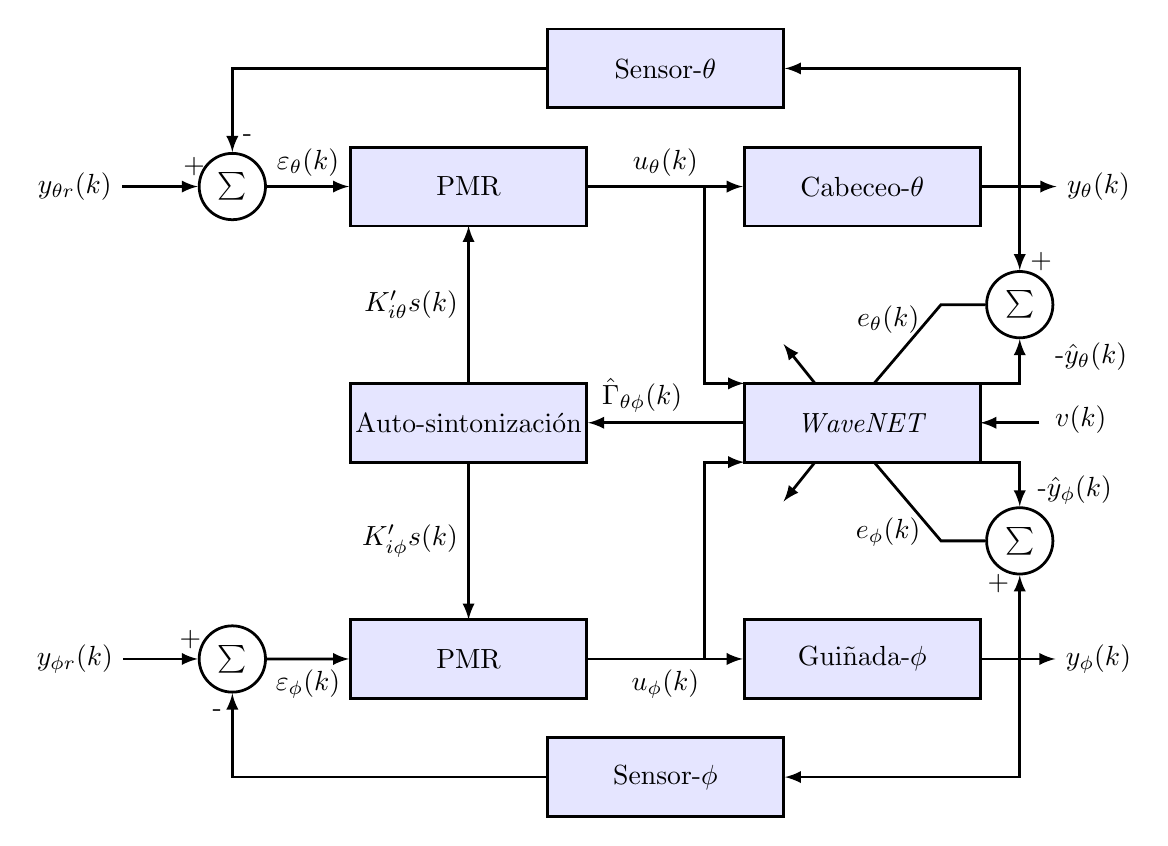
\begin{tikzpicture}[node distance = 5cm, auto, >=latex, line width = 1pt]
    \tikzstyle{block} = [draw, fill = blue!10, shape = rectangle, inner sep = 1pt, minimum height = 1cm, minimum width = 3cm]
    \tikzstyle{sum} = [draw, shape = circle, minimum size = 1em]

    \node[sum] (begin) at (0,0) {$\sum$};
    \node[] (start) [left of = begin, node distance = 2cm] {$y_{\theta r}(k)$};
    \node[block] (control) [right of = begin, node distance = 3cm] {PMR};
    \node[block] (process) [right of = control] {Cabeceo-$\theta$};
    \node[] (end) [right of = process, node distance = 3cm] {$y_{\theta}(k)$};
    \node[block] (gains) [below of = control, node distance = 3cm] {Auto-sintonización };
    \node[block] (rna) [below of = process, node distance = 3cm] {\textit{WaveNET}};
    \node[sum] (sum) at (10,-1.5) {$\sum$};
    \node[block] (sensor) at (5.5,1.5) {Sensor-$\theta$};
    
    \draw[->] (start) -- node[pos = 0.95] {+} (begin);
    \draw[->] (begin) -- node[pos = 0.50] {$\varepsilon_{\theta}(k)$} (control);
    \draw[->] (control) -- node {$u_{\theta}(k)$} (process);
        
    \draw[->] (3,-2.5) -- node {$K'_{i\theta}s(k)$} (3,-0.5);
    \draw[->] (10,0) -- node[pos = 0.9] {+} (sum);
    \draw[->] (9.25,-2.5) -| node[pos = 0.80, xshift = 1.5cm] {-$\hat{y}_{\theta}(k)$} (sum);
    \draw[->] (6.00,0) |- (6.5,-2.5);
    \draw[->] (10.25,-3) -- node[xshift = 0.90cm, yshift = 0.35cm]{$v(k)$} (9.5,-3);
    \draw[- ] (sum) -- (9,-1.5) -- node[pos = 0.5, above, xshift = -7pt]
        {$e_{\theta}(k)$} (8.15,-2.5);
    \draw[->] (7.4,-3.5) -- (7,-4);
    \draw[->] (10,0) |- (sensor);
    \draw[->] (sensor) -| node[pos = 0.9] {-} (begin);
    \draw[->] (process) -- (end);
    \draw[->] (rna) -- node[pos = 0.65, above] {$\hat{\Gamma}_{\theta\phi}(k)$} (gains);
    
    \node[sum] (begin2) at (0,-6) {\tiny $\sum$};
    \node[] (start2) [left of = begin2, node distance = 2cm] {$y_{\phi r}(k)$};
    \node[block] (control2) [below of = gains, node distance = 3cm] {PMR};
    \node[block] (process2) [below of = rna, node distance = 3cm] {\centering Guiñada-$\phi$};
    \node[] (end2) [right of = process2, node distance = 3cm] {$y_{\phi}(k)$};
    \node[block] (sensor2) at (5.5,-7.5) {Sensor-$\phi$};
    \node[sum] (sum2) at (10,-4.5) {$\sum$};
    
    \draw[<-] (3,-5.5) -- node {$K'_{i\phi}s(k)$} (3,-3.5);
    \draw[->] (start2) -- node[pos = 0.90] {+} (begin2);
    \draw[->] (begin2) -- node[pos = 0.50, below] {$\varepsilon_{\phi}(k)$} (control2);
    \draw[->] (control2) -- node[below] {$u_{\phi}(k)$} (process2);
    \draw[->] (6,-6) |- (6.5,-3.5);
    \draw[->] (10,-6) -- node[pos = 0.90] {+} (sum2);
    \draw[->] (9.25,-3.5) -| node[pos = 0.80, xshift = 0.7cm, below, yshift = 0.3cm] {-$\hat{y}_{\phi}(k)$} (sum2);
    \draw[->] (10,-6) |- (sensor2);
    \draw[->] (sensor2) -| node[pos = 0.90] {-} (begin2);
    \draw[->] (process2) -- (end2);
    
    \draw[- ] (sum2) -- (9,-4.5) -- node[pos = 0.5, above, xshift = -7pt, yshift = -0.7cm] {$e_{\phi}(k)$} (8.15,-3.5);
    \draw[->] (7.4,-2.5) -- (7,-2);
\end{tikzpicture}}
        \caption[Diagrama de bloques de los controladores PMR.]{Diagrama de bloques de los controladores proporcionales multiresolución.}
        \label{fig:schematicControlPMR}
    \end{figure}
        
     En palabras de \citeauthor{VegaNavarrete2013}, la señal de error se descompone en señales a diferentes niveles, la cuales se escalan con sus respectivas ganancias y al ser sumadas se obtiene la señal de control, que está expresada por \cite[p. 43]{VegaNavarrete2013} la siguiente ecuación
    \begin{equation}
        u(k) = \sum\limits_{i=1}^{N+1} K_i \varepsilon_i(k)
    \end{equation}
    \begin{eqexpl}
        \item{$N$} indica el nivel de resolución, 
        \item{$\varepsilon_i$} es la señal de error de la $i$-ésima escala, y
        \item{$K_i$} representa la ganancia para cada $i$-ésimo componente.
    \end{eqexpl}
        
        % Si se toma como ejemplo el control \acrshort{pid} discreto y recordando la \cref{equa:getsignal.vi} que proporciona su señal de control,
        
    Se puede indicar la nueva expresión que utilice el enfoque de multiresolución, es decir
    \begin{equation}
        u_{k+1} = u_{k} + \sum\limits_{i=1}^{3} K_i \varepsilon_{k(i)}
    \end{equation}
    \begin{eqexpl}
        \item{$k$}específica la época, y
        \item{$\sum$}se limita a tres, pues es la cantidad de componentes en el contraloador PID.
    \end{eqexpl}
        
    Como ya se dijo antes, la configuración del control PMR tiene la característica de emplear dos o más parámetros que dependen del nivel de resolución aplicada a la señal de error; la \cref{fig:structurePMR} muestra el diagrama empleado, mientras que el bloque de descomposición se ilustra en la \cref{fig:structure3levelsDescomp}.

    \begin{figure}[H]
        \centering
        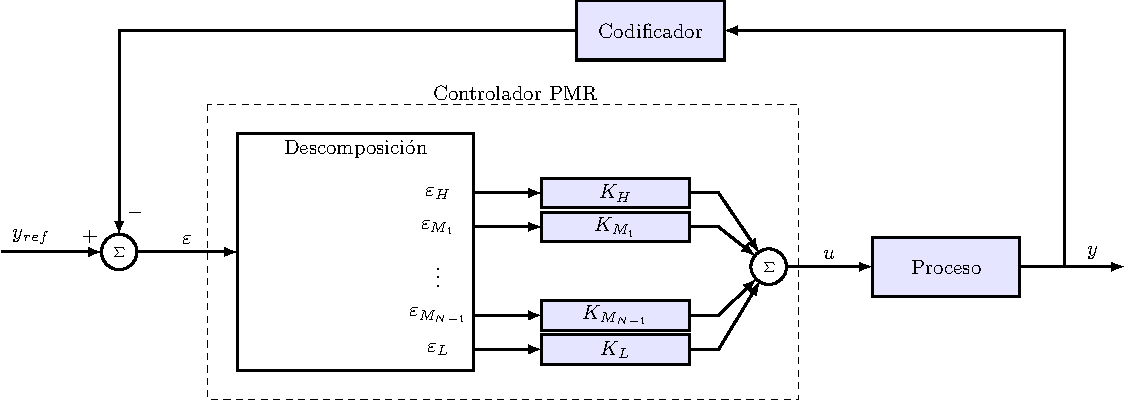
\includegraphics[width = \textwidth]{graphics/pmr/Block PMR Structure.pdf}
        \caption[Diagrama del controlador PMR en lazo cerrado.]{Diagrama del controlador PMR en lazo cerrado \cite[p. 48]{VegaNavarrete2013}.}
        \label{fig:structurePMR}
    \end{figure}
        
    \begin{figure}[H]
        \centering
        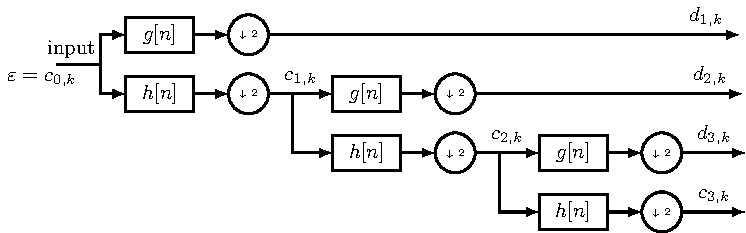
\includegraphics[width = 0.8\textwidth]{graphics/pmr/Filter Descomp 3 Levels.pdf}\\ \vspace*{0.5em}
        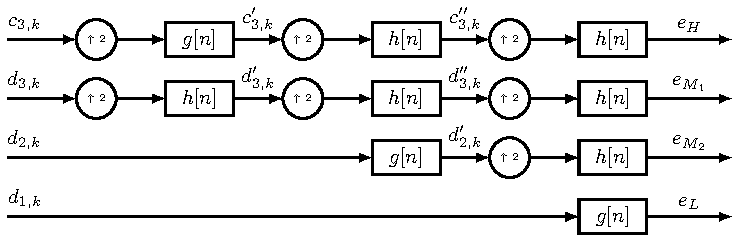
\includegraphics[width = 0.8\textwidth]{graphics/pmr/Filter Sint 3 Levels.pdf}
        \caption[Diagrama de análisis de tres niveles.]{Diagrama de descomposición y síntesis de tres niveles \cite[p. 47]{VegaNavarrete2013}.}
        \label{fig:structure3levelsDescomp}
    \end{figure}
        
     La expresión general para escalar los componentes es
    \begin{align}
        u &= K_{H}\varepsilon_{H} + K_{M_1}\varepsilon_{M_1} + \cdots + K_{i}\varepsilon_{i} + \cdots + K_{L}\varepsilon_{L}
    \end{align}
    que expresándola en su forma matricial se tiene
    \begin{align}
        u &= \mathbf{K}\odot\mathbf{E_m},\,\text{siendo} \\
        \mathbf{K} &= 
            \begin{bmatrix}
                K_{H} & K_{M_1} & \cdots & K_{i} & \cdots & K_{L}
            \end{bmatrix},\,\text{y}\\
        \mathbf{E_m} &= 
            \begin{bmatrix}
                \varepsilon_{H} & \varepsilon_{M_1} & \cdots & \varepsilon_{i} & \cdots & \varepsilon_{L}
            \end{bmatrix}.
    \end{align}
        
    Finalmente, \citeauthor{VegaNavarrete2013} presenta las reglas de sintonización automática, las cuales están implícitas en las leyes del control anterior, por lo tanto se tiene
    \begin{align}
        K_{H}[k+1] &= (K_{H}[k]T + \mu_{H} \hat{\Gamma} (\varepsilon_H[k] - \varepsilon_H[k]))/T \\
        K_{M_1}[k+1] &= (K_{M_1}[k-1]T + \mu_{M_1} \hat{\Gamma} (\varepsilon_{M_1}[k] - \varepsilon_{M_1}[k-1]))/T \\
        &\vdots \\
        K_{M_{N-1}}[k+1] &= (K_{M_{N-1}}[k-1]T + \mu_{M_{N-1}} \hat{\Gamma} (\varepsilon_{M_{N-1}}[k] - \varepsilon_{M_{N-1}}[k-1]))/T \\
        K_{L}[k+1] &= (K_{L}[k-1]T + \mu_{L} \hat{\Gamma} (\varepsilon_L[k] - \varepsilon_L[k-1]))/T
    \end{align}
    donde
    \begin{align}
        \Gamma[k] &= \sum\limits_{i=0}^{M} c_i z[k-i]u[k]
    \end{align}
    y las $\mu$ se tratan de la taza de actualización o aprendizaje del controlador.

        % Los resultados obtenidos en la \cref{sec:ident_fOut} fueron tomados como base, pues la configuración encontrada para la \textit{wavenet} ya cuenta con el entrenamiento, entonces sólo fue necesario realizar la operación dentro de línea para hallar los parámetros del nuevo controlador.
\section{Identificación fuera línea}\label{sec:PMR_outline}
        
\section{Identificación en línea}\label{sec:PMR_online}
    \initchapterlong
    {Diseño de la interfaz cerebro-computadora}
    {Diseño de la interfaz cerebro-\\computadora}\label{chap:design bci}
    \include{mainmatter/conclusion}
    
    % ============================================================
    % THESIS CONTENT - APPENDICES
    % ============================================================
    \appendix
    \appendixsetup
    
    % Rename appendix name PDF
    \makeatletter
        \bookmarksetup{
            addtohook = {
                \ifnum\toclevel@chapter = \bookmarkget{level}\relax
                    \renewcommand*{\numberline}[1]{\appendixname~#1.~}
                \fi
            },
        }
    \makeatother
    \include{appendices/modelmath}
    
    % ============================================================
    % BIBLIOGRAPHY
    % ============================================================
    % \nocite{*}
    \nocite{Siuly2017}
    \headerEmpty{Referencias}
    \printbibliography[ title   = Referencias,
                        heading = bibintoc]
    % }
    % ============================================================
    % BACKMATTER: ABBREVIATIONS, ACRONYMS, GLOSSARIES, NOTATION
    % ============================================================
    \bookmarksetup{startatroot}
    \pagelinknum
    \printnomenclature[3cm]
    \headerEmpty{Notación}
    \addcontentsline{toc}{chapter}{\nomname}
    
    % \glsaddall
    \printglossary[type  = \acronymtype,
                   title = Acrónimos y abreviaturas, 
                   style = super]
    \headerEmpty{Acrónimos y abreviaturas}
    
    % \printglossary
    % \headerEmpty{Glosario}
% ================================================================
% ================================================================
\end{document}
% ================================================================